\documentclass[10pt,utf8]{beamer}

\mode<presentation> {
%  \usetheme{Boadilla}
  \usetheme{Madrid}
%	\usetheme{Fzu}
  \setbeamercovered{transparent}
}

\usepackage{palatino}
\usepackage{graphicx}
\usepackage{array}
\usepackage{color}
\usepackage{subfigure}
\usepackage{colortbl}
\usepackage{amsmath}
\usepackage{hyperref}
\usepackage{listings}
\usepackage{fancyvrb}

\setbeamertemplate{caption}{\raggedright\insertcaption\par} %turn off caption prefix ("Figure")

\title{Disk Paxos and Delta Leases}
\author{Vojtech Juranek}
\institute[Red Hat]{Red Hat}
\date{22.~10.~2019}

\lstdefinestyle{Bash}{
	basicstyle          = \large\ttfamily,
	language            = Bash,
	numbers             = left,
	numberstyle         = \small,
	stepnumber          = 1,
	numbersep           = 5pt,
	backgroundcolor     = \color{white},
	showspaces          = false,
	showstringspaces    = false,
	showtabs            = false,
	frame               = single,
	tabsize             = 2,
	captionpos          = b,
	breaklines          = true,
	breakatwhitespace   = false,
	morestring          = [b]",
	stringstyle         = \color{blue},
	keywordstyle        = \color{magenta},
	commentstyle        = \color{gray},
	identifierstyle     = \color{black},
	moredelim           = **[is][\bfseries]{`}{`},
	moredelim           = **[is][\color{magenta}]{!}{!}, 
	fancyvrb            = true,
}


\begin{document}

\begin{frame}
    \titlepage
\end{frame}

\begin{frame}
    \frametitle{Network attached storage}
    \begin{figure}
        \centering
        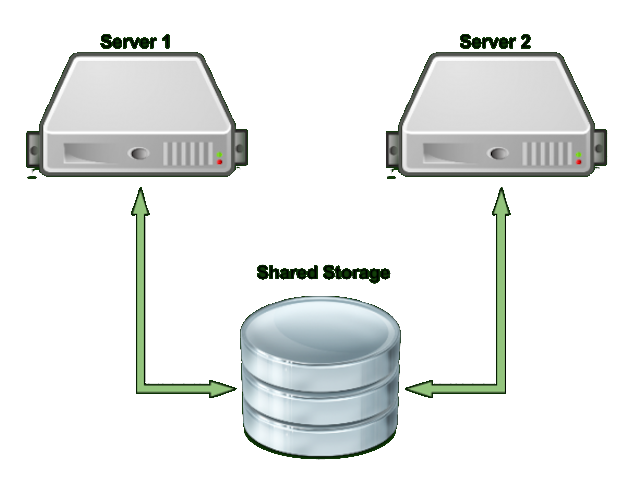
\includegraphics[height=5cm]{./img/disk-paxos.eps}
        \caption{\tiny{Source: \url{https://www.linuxjournal.com/content/high-availability-storage-ha-lvm}}}
    \end{figure}
\end{frame}

\begin{frame}
    \frametitle{Storage area network}
    \begin{figure}
        \centering
        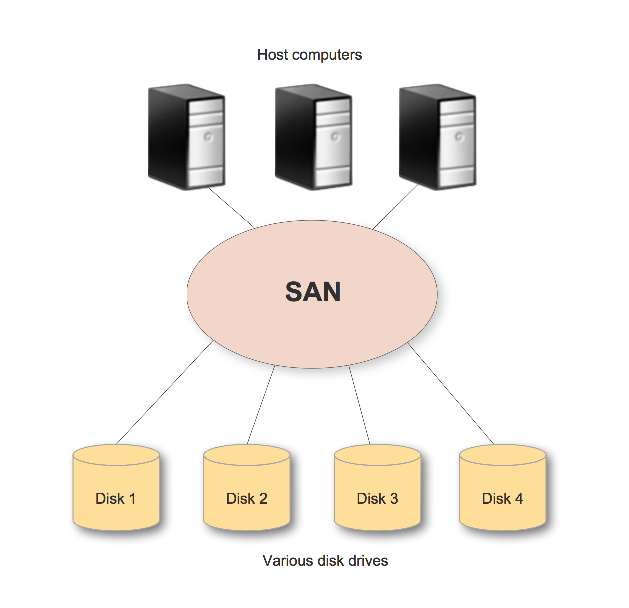
\includegraphics[height=7cm]{./img/san.eps}
        \caption{\tiny{Source: \url{https://www.ibm.com/developerworks/community/wikis/
        %\caption{\tiny{Source: \url{https://www.ibm.com/developerworks/community/wikis/home?lang=en\#!/wiki/IBM\%20Technology\%20Made\%20Simple/page/Storage\%20Virtualization\%20Technology
        }}}
    \end{figure}
\end{frame}

\begin{frame}
    \frametitle{Storage virtualization}
    \begin{figure}
        \centering
        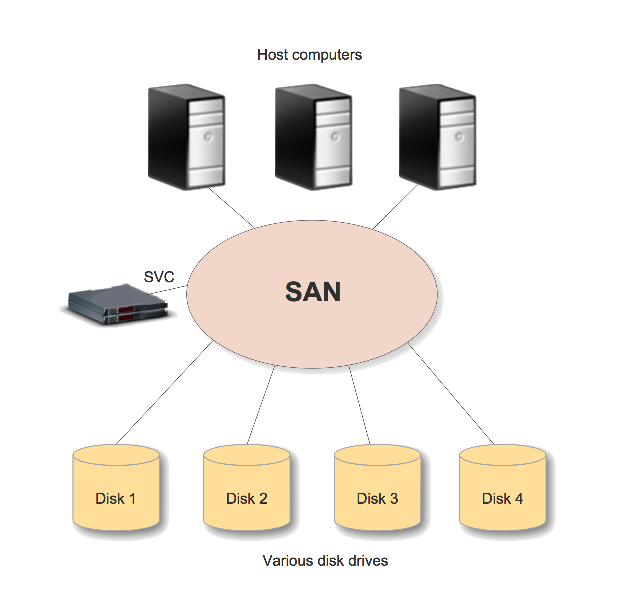
\includegraphics[height=7cm]{./img/san-svc.eps}
        \caption{\tiny{Source: \url{https://www.ibm.com/developerworks/community/wikis/
        %\caption{\tiny{Source: \url{https://www.ibm.com/developerworks/community/wikis/home?lang=en\#!/wiki/IBM\%20Technology\%20Made\%20Simple/page/Storage\%20Virtualization\%20Technology
        }}}
    \end{figure}
\end{frame}

\begin{frame}
    \frametitle{Storage virtualization}
    \begin{figure}
        \centering
        
\includegraphics[height=5cm]{./img/virt-storage.eps}
        \caption{\tiny{Source: \url{https://sharedstorage.wordpress.com/2017/01/03/storage-virtualization/}}}
    \end{figure}
\end{frame}

\begin{frame}
    \frametitle{Refresh: Consensus algorithm}
    \centering
    \textbf{Algorithm has to satisfy 2 conditions:}
    \vspace{0.5cm}
    \begin{itemize}
     \item safety (consistency)
     \item liveness (non-blocking)
    \end{itemize}
\end{frame}

\begin{frame}
    \frametitle{Refresh: Classic Paxos}
    \centering
    \textbf{3-phase commit protocol called Synod:}
    \vspace{0.5cm}
    \begin{itemize}
     \item voting
     \item prepare to commit (pre-commit)
     \item commit
    \end{itemize}
\end{frame}

\begin{frame}
    \frametitle{Refresh: Basic Paxos}
    \begin{figure}
        \centering
        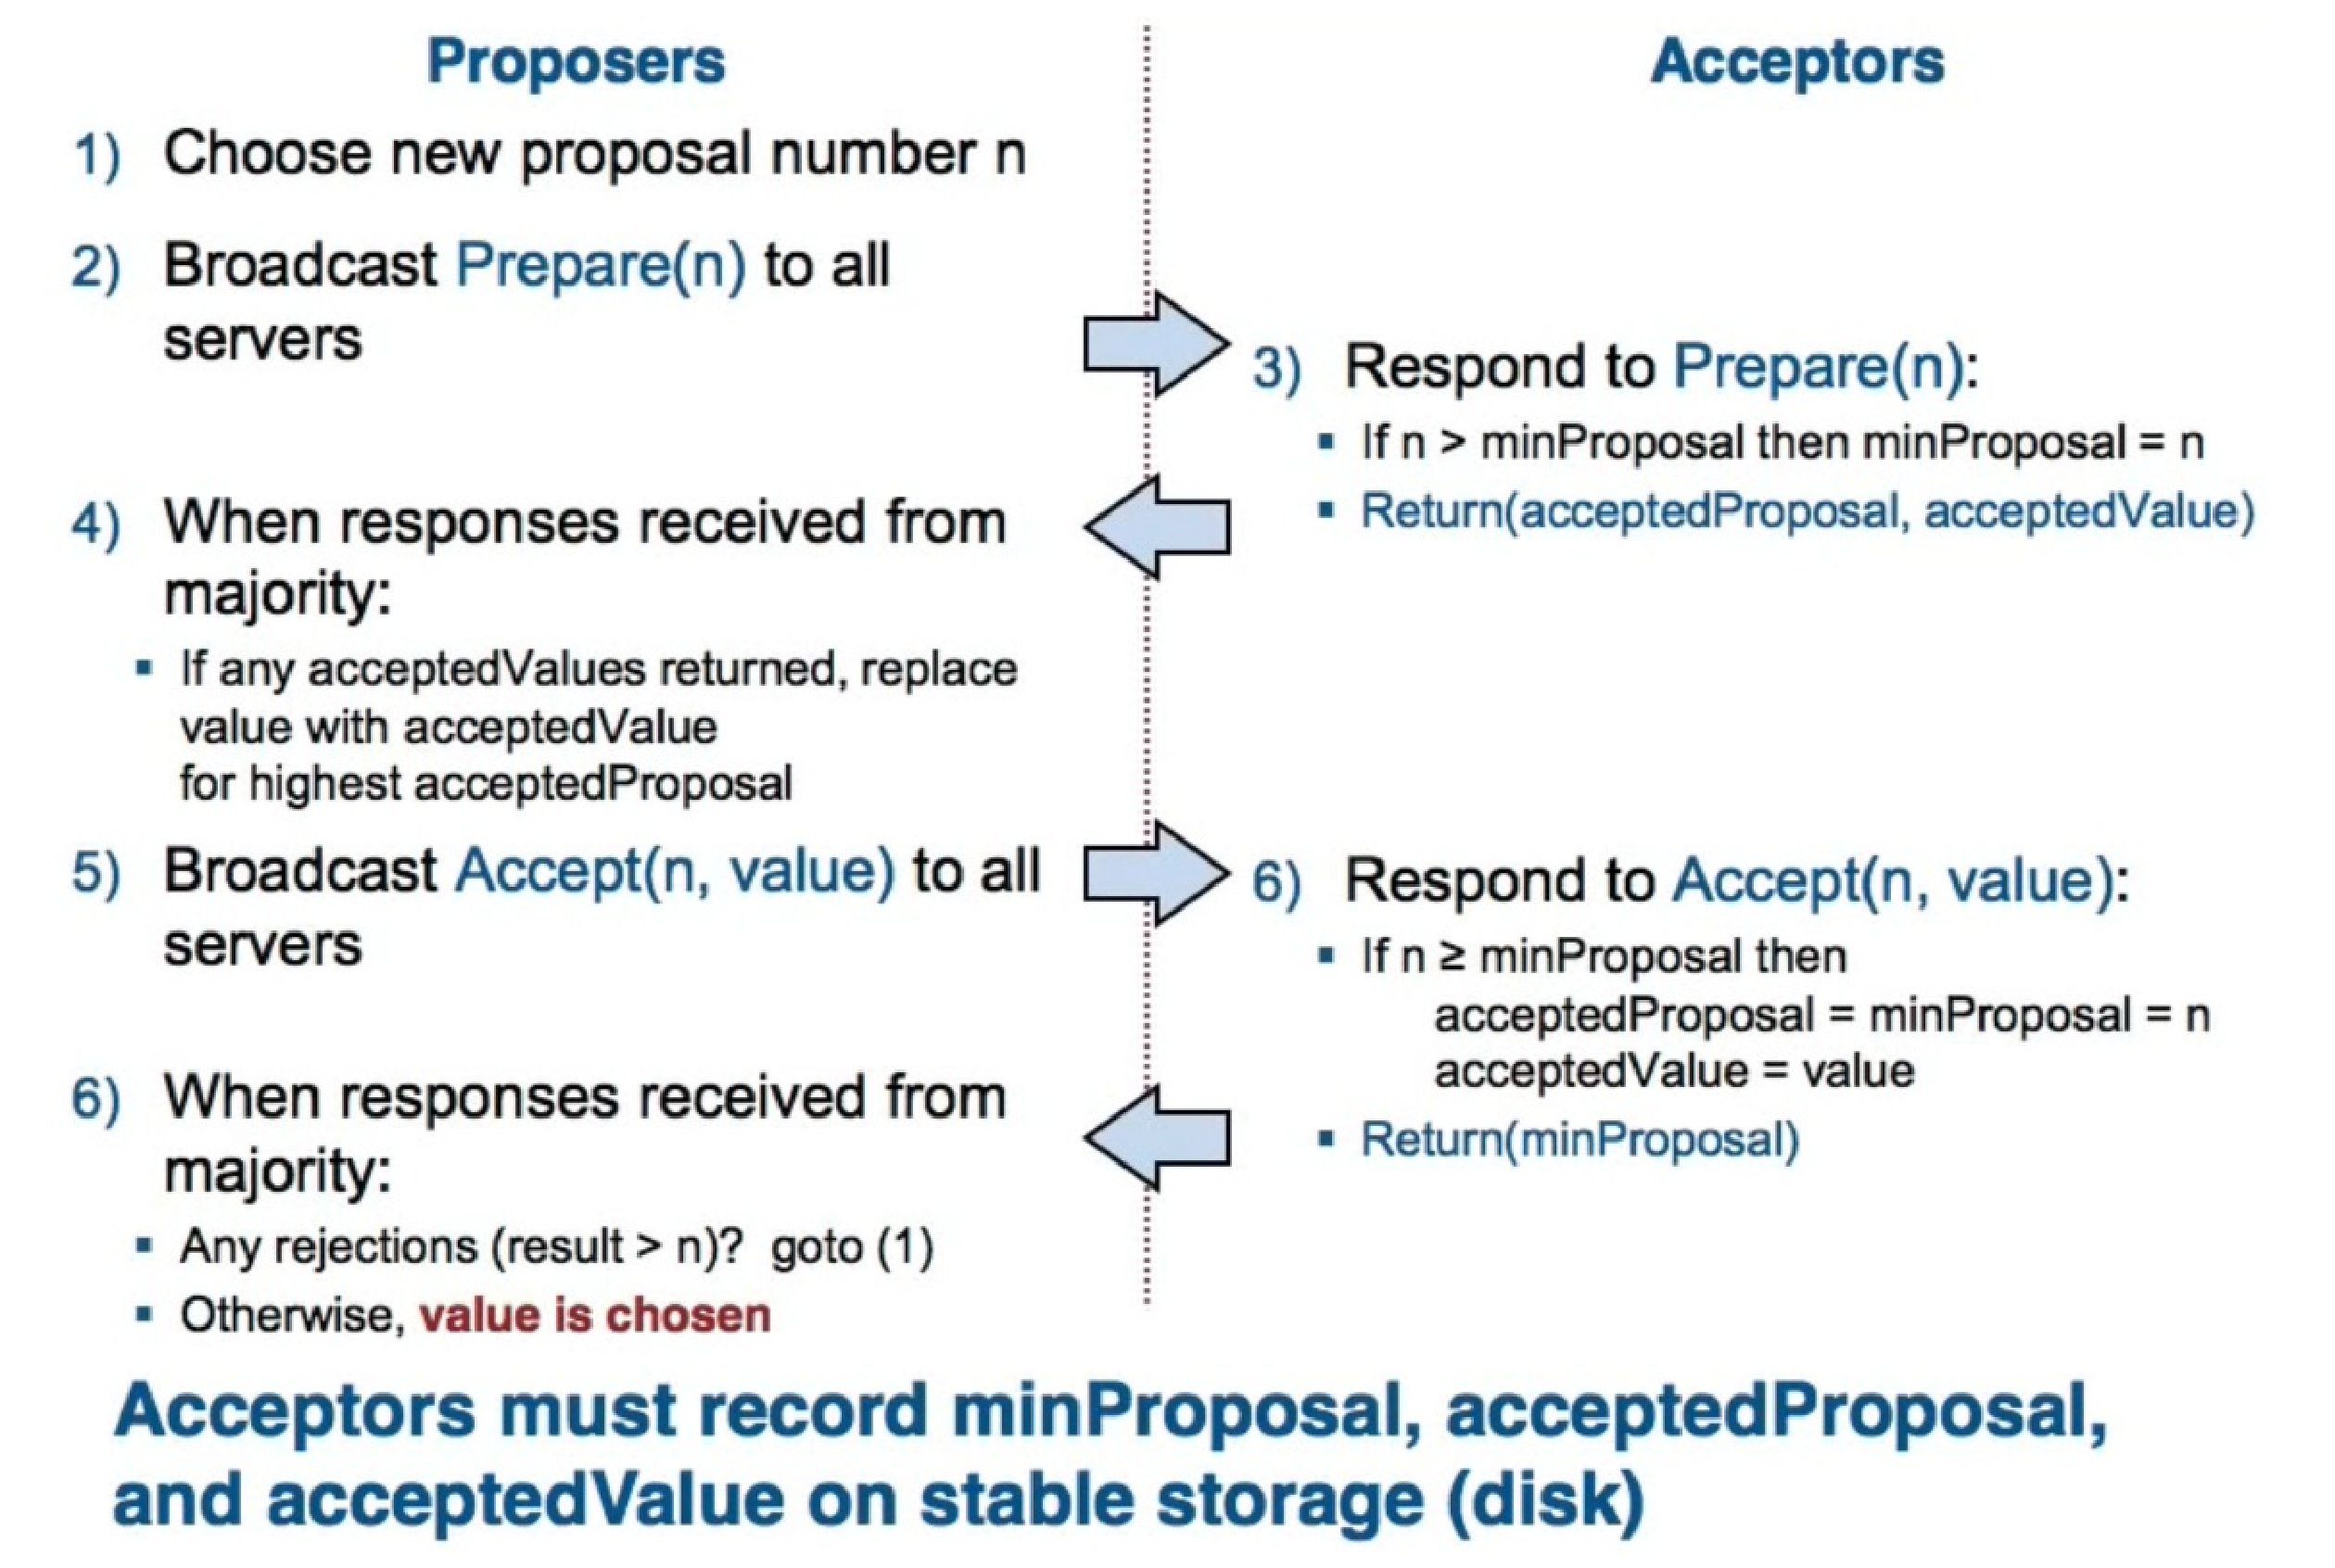
\includegraphics[height=7cm]{./img/basic-paxos.eps}
        \caption{\tiny{Source: \url{https://youtu.be/JEpsBg0AO6o?t=1050}}}
    \end{figure}
\end{frame}

\begin{frame}
    \frametitle{Disk Paxos}
    \begin{figure}
        \centering
        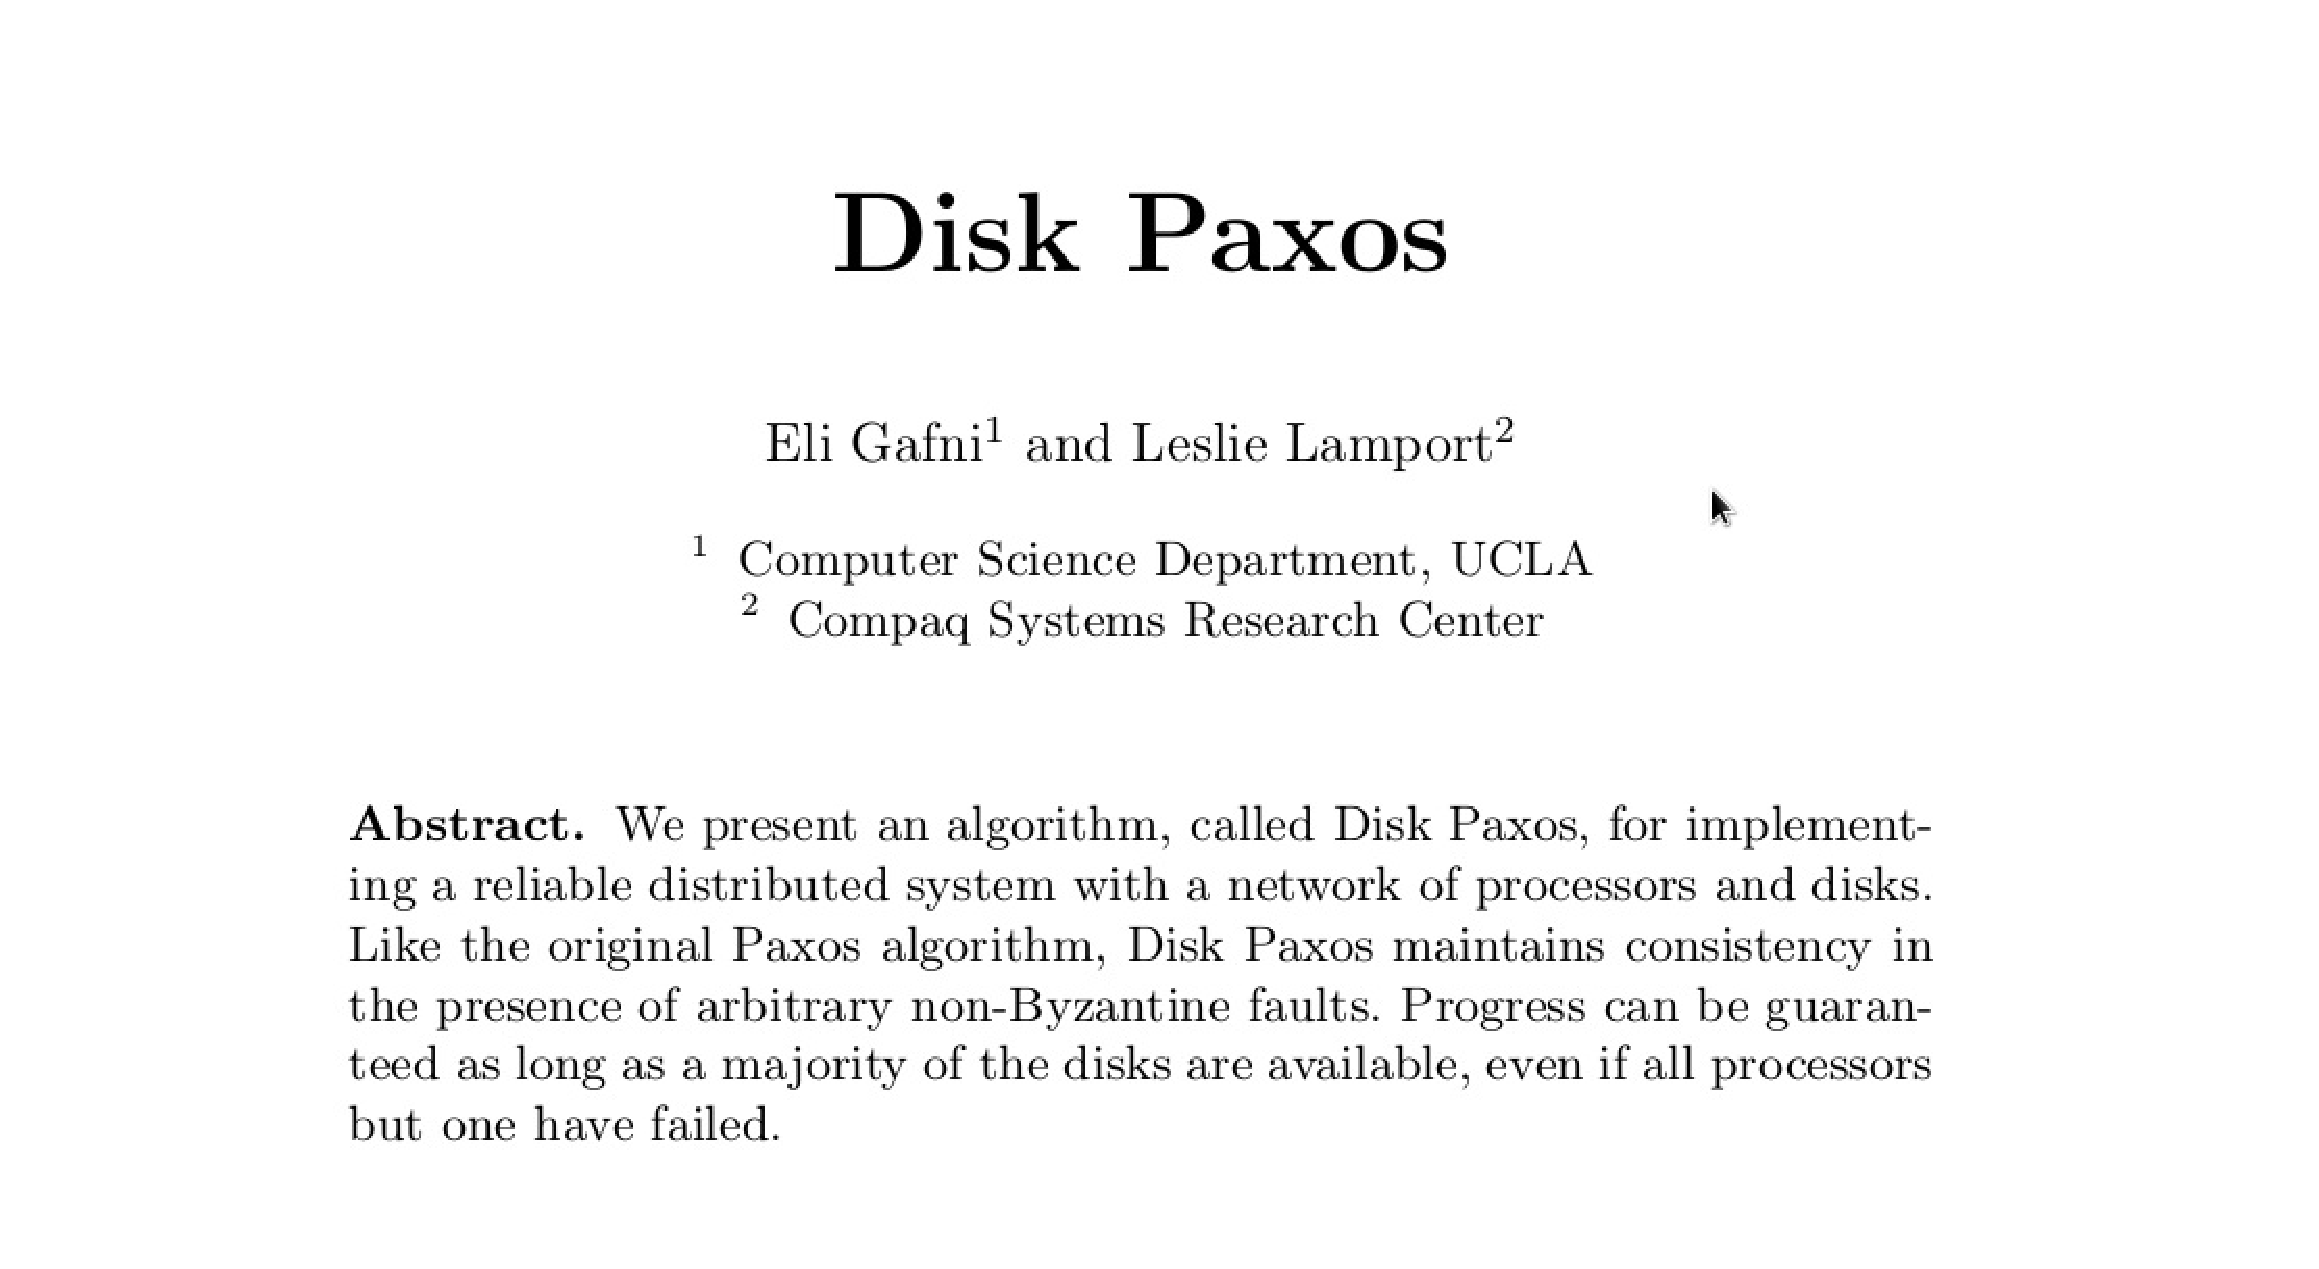
\includegraphics[height=5cm]{./img/disk-paxos-paper.eps}
    \end{figure}
\end{frame}

\begin{frame}
    \frametitle{Disk Paxos}
    \centering
    \textbf{Two main phases:}
    \vspace{0.5cm}
    \begin{itemize}
     \item proposing a value
     \item preparing the commit of a value
    \end{itemize}
\end{frame}


\begin{frame}
    \frametitle{Disk Paxos}
    \centering
    \textbf{In whole algorithm we assume reading and writing are atomic operations.}\\
    \vspace{1cm}
    
    \begin{itemize}
     \item Each processor has an assigned block on each disk.
     \item Stores following structure \texttt{dblock[p]}:
     \begin{itemize}
        \item \texttt{mbal} - ballot number
        \item \texttt{bal} - largest ballot number for which \texttt{p} reached preparing commit phase
        \item \texttt{inp} - value \texttt{p} tries to commit in ballot \texttt{bal}
     \end{itemize}
    \end{itemize}
\end{frame}


\begin{frame}
    \frametitle{Phase 1: proposing a value}
    \centering
    \textbf{For each disk \texttt{d}}
    \vspace{0.5cm}
    \begin{itemize}
        \item write \texttt{dblock[p]} to disk \texttt{[d][p]}
        \item read \texttt{dblock[p]} from \texttt{[d][q]} for all other processes \texttt{[q]}
    \end{itemize}
    
    \vspace{1cm}
    
    \centering
    \textbf{For any disk \texttt{d} and process \texttt{q}:}
    \vspace{0.5cm}
    \begin{itemize}
        \item if \texttt{[d][q].mbal > dblock[p].mbal} $\rightarrow$ abort
        \item else if read majority of disks $\rightarrow$ phase finished
    \end{itemize}
\end{frame}

\begin{frame}
    \frametitle{Phase 2: preparing the commit of a value}
    \centering
    \textbf{Choosing a value:}
    \vspace{0.5cm}
    \begin{itemize}
     \item \texttt{inp = dblock[q].inp}, where \texttt{dblock[q]} is block with largest \texttt{dblock[q].bal} among read blocks
     \item or value proposed by \texttt{p} is all read blocks haven't any value set
    \end{itemize}
\end{frame}

\begin{frame}
    \frametitle{Phase 2: preparing the commit of a value}
    
    \centering
    \textbf{For each disk \texttt{d}}
    \vspace{0.5cm}
    \begin{itemize}
        \item write \texttt{dblock[p]} to disk \texttt{[d][p]}
        \item read \texttt{dblock[p]} from \texttt{[d][q]} for all other processes \texttt{[q]}
    \end{itemize}
    
    \vspace{1cm}
    
    \centering
    \textbf{For any disk \texttt{d} and process \texttt{q}:}
    \vspace{0.5cm}
    \begin{itemize}
        \item if \texttt{[d][q].mbal > dblock[p].mbal} $\rightarrow$ abort and start phase 1 with higher ballot number
        \item else if read majority of disks $\rightarrow$ value committed, broadcast it
    \end{itemize}
\end{frame}

\begin{frame}
    \frametitle{Broadcasting a value}
    
    \centering
    \textbf{If \texttt{p} learns that some other value was committed during the process $\rightarrow$ abort and output committed value.}
\end{frame}


\begin{frame}
    \frametitle{Delta leases}
    \begin{figure}
        \centering
        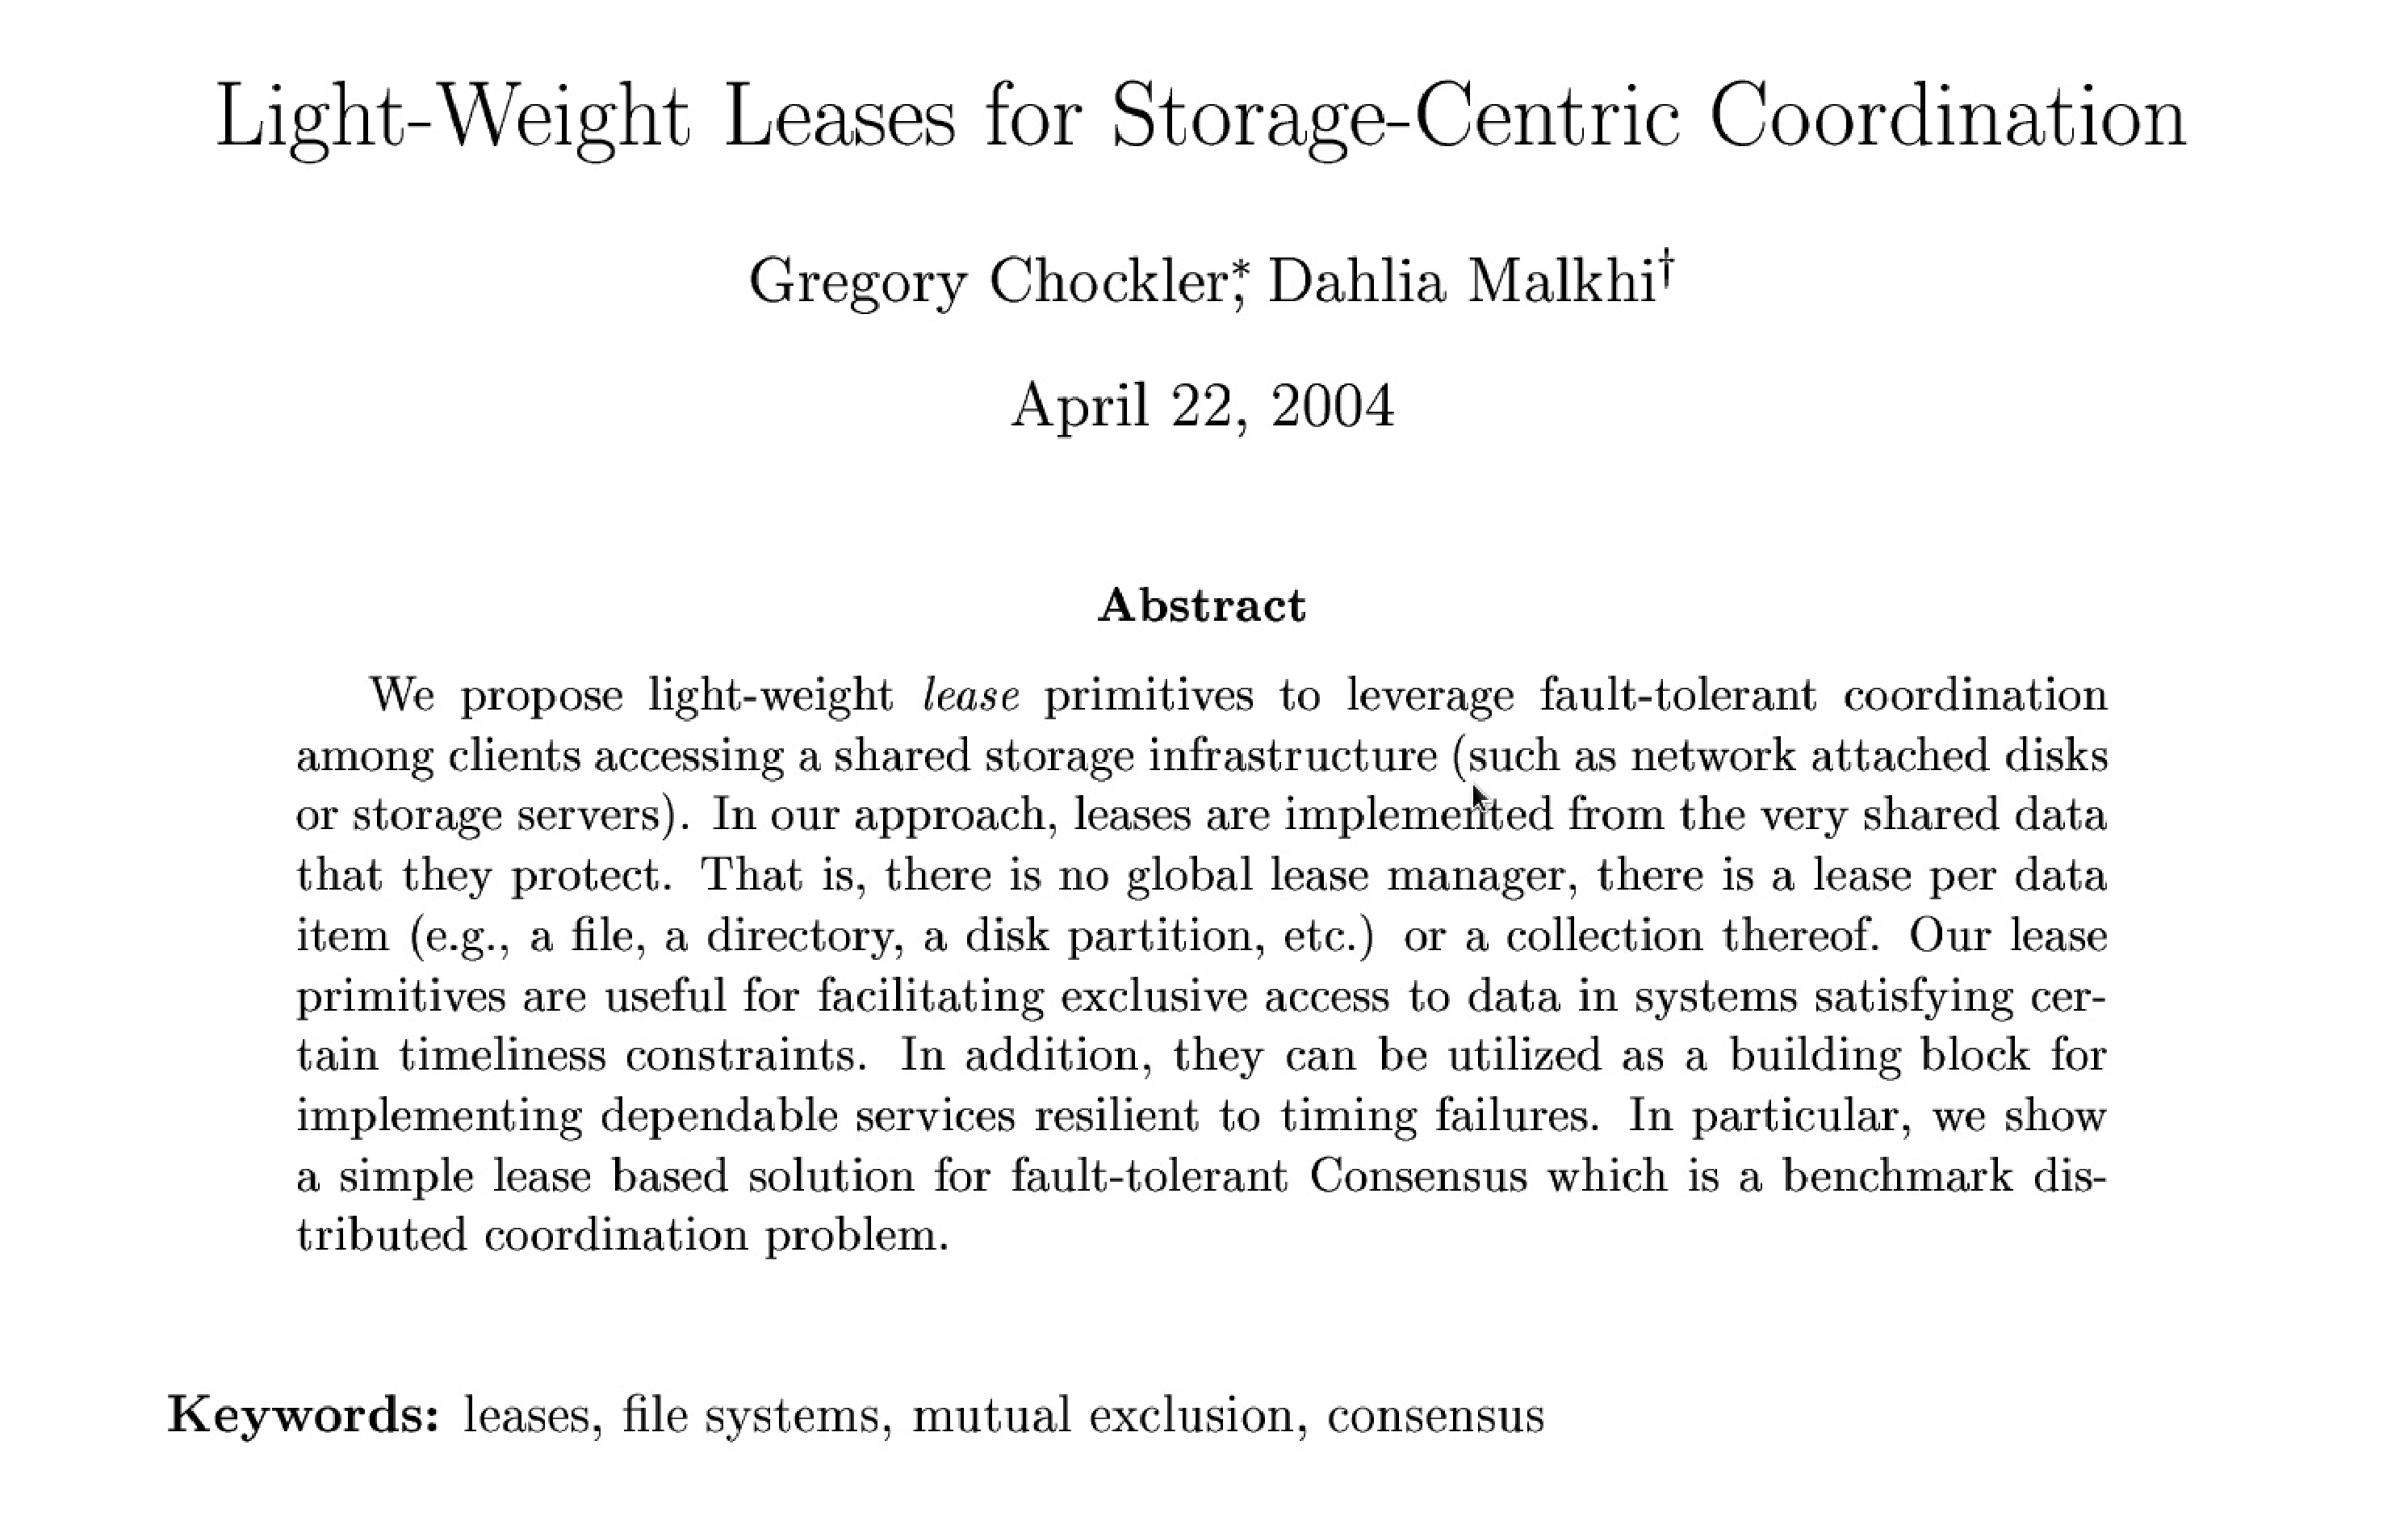
\includegraphics[height=5cm]{./img/delta-leases-paper.eps}
    \end{figure}
\end{frame}

\end{document}
